\documentclass[11pt, a4paper, main=english, ngerman, footlines=1, footheight=14pt]{scrreprt}

% You can enable the following options while you write. Please disable them in the final version.
\usepackage[
    coloredrefs,                % references are colored blue
    notes,                      % notes helpers
    % grid,                        % show grid and layout frames
    % pagebreaks                   % break page before every section, sub-section and sub-sub-section
]{template/template}
\usepackage{template/custom_commands}    % custom commands
\usepackage{template/custom_listings}    % custom code languages for listings
\usepackage{data}               % contains setters for all information required, such as title, names, etc.
\usepackage[textsize=small]{todonotes}
\setuptodonotes{inline}
\usepackage{hyperref} % For customref
%TODO FIX:
\glsdisablehyper  %keine hyperlinks weil kein glossar


\makeglossaries
\loadglsentries{parts/_acronyms}
\loadglsentries{parts/_glossary}

% If you use TikZ, you can define the required libraries here. Example:
% \usetikzlibrary{arrows, automata}


\begin{document}

% Title page
\input{\getTitlepageFile}

% Intro
\beginIntro

\addcontentsline{toc}{chapter}{\protect\numberline{}\langPreface}

\getStatements

% Content lists
\newpage
\addcontentsline{toc}{section}{\langTableOfContents}

% Content lists
% TODO: comment out the ones not needed
\tableofcontents            \vspace{1.5\baselineskip}
\listoffigures              \vspace{1.5\baselineskip}
\listoftables               \vspace{1.5\baselineskip}
\lstlistoflistings          \vspace{1.5\baselineskip}
\listofacronyms             \vspace{1.5\baselineskip}
\myglossary

% Content
\beginContent
\chapter{Implementation}

\section{Design Discussion}

Before settling on the final master-worker tile decomposition, we discussed several alternative designs for the key open questions below.

\subsection{Tile Distribution}
\begin{itemize}
    \item Dynamic tile allocation (as opposed to a static, fixed split of work per process) was already given to us as a requirement of the assignment,the question for us was how to implement it.
    \begin{itemize}
        \item The master pre-computes the full list of tiles for the image (row-major scan order) once, up front.
        \item Tiles are then handed out dynamically, one at a time, as each worker becomes idle, rather than pre-assigning a fixed share of tiles to each worker.
        \item This addresses the static row-decomposition imbalance we discussed in Assignment 2, where a fixed, equal split of work per rank did not account for the image size not dividing evenly among processes.
    \end{itemize}
\end{itemize}

\subsection{Discussion 1- Assembling the Final Image}
\begin{itemize}
    \item How would workers report finished tiles back to the master so it can assemble the final output? We discussed two options:
    \begin{itemize}
        \item \textbf{Version 1:} each worker allocates a vector the size of the \emph{entire} final image. As it receives tiles, it writes each rendered tile into its correct position in that full-size buffer, leaving the rest unused. At the end, all workers' buffers are combined into the master's final image with a single collective \texttt{MPI\_Gather}/\texttt{MPI\_Gatherv} call.
        \item \textbf{Version 2:} each worker only ever holds the data for the one tile it is currently responsible for, together with that tile's coordinates/dimensions. Results are sent back and collected via \texttt{MPI\_Gather} at the end, instead of each worker carrying a full-image-sized buffer the whole time.
    \end{itemize}
    \item Version 2 was preferred: it avoids every worker allocating a full-image-sized buffer (wasteful memory-wise, especially as process count grows and most of each buffer would stay empty), and keeps the data a worker holds proportional to the tile it is actually working on.
\end{itemize}

\subsection{Discussion 2- Work Queue Implementation}
\begin{itemize}
    \item How should the dynamic tile queue be implemented?
    \begin{itemize}
        \item \textbf{Option 1 -- shared memory queue:} we first discussed exposing the tile queue as a shared-memory structure that all workers could pull from directly, using MPI-3's one-sided \texttt{MPI\_Win\_allocate\_shared} windows~\cite{mpi31_standard}.
        \item This was dropped though- as when Ilhom was implementing it - he found out it to be more complicated than necessary (processes do not share an address space by default in MPI) and would require more complex mechanisms (manual synchronization over the shared window) to implement properly.
        \item \textbf{Option 2 -- message passing (chosen):} the master holds the authoritative tile list and queue state itself, and workers request/receive tiles purely via point-to-point messages (\texttt{MPI\_Send}/\texttt{MPI\_Recv}). This is a centralized work queue distributed through message passing, not a genuinely shared queue in the memory-sharing sense -- which avoids the synchronization complexity of Option 1.
    \end{itemize}
\end{itemize}

\subsection{Snowflake Generation Granularity}
\begin{itemize}
    \item We realized with the original implementation we would regenerate the snowflake field for every tile a worker renders.
    \item This would couple the total amount of work to the number of tiles: more tiles would mean the snowflake field gets regenerated more often, directly working against the goal of using small tiles for good load balancing.
    \item To avoid this, snowflake generation was separated from tile rendering- now we have each worker generate the snowflake field exactly once (75{,}000 points, fixed seed so every worker produces the identical field), covering the whole image, before it starts processing any tiles -- not once per tile and not once per row.
\end{itemize}

\chapter{Evaluation}
\section{Strong scaling}

\begin{figure}
    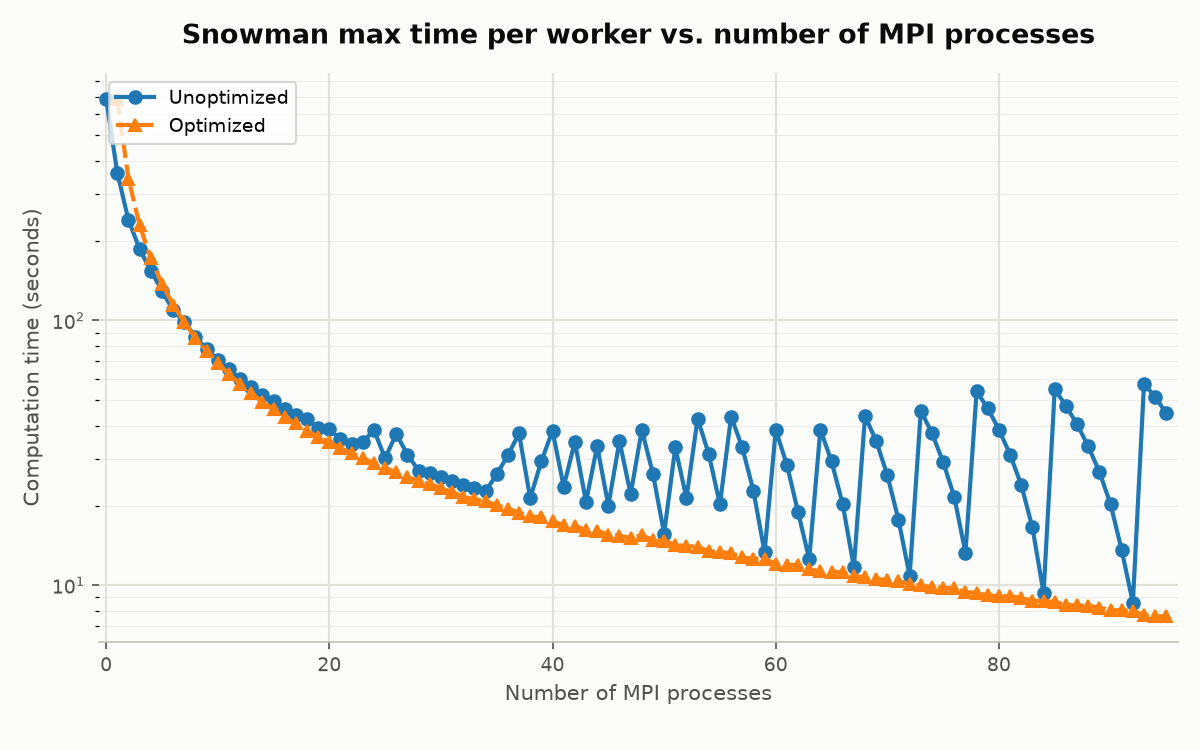
\includegraphics[width=\textwidth]{parts/images/max_times_comparison.png}
    \caption{Runtime for 1 to 96 MPI processes}
\end{figure}

Figure 2.1 shows the runtimes of the optimized and unoptimized code for 1 to 96 MPI processes. A logarithmic scale is used, so differences in the lower runtimes can be seen more clearly. The spikes in runtime of the unoptimized code come from the way the remainder is handled when the rows of the image can not be evenly distributed among the processes: the entire remainder is given to the last process, leading to an uneven distribution of work. Using our tile decomposition, these spikes disappear. This is because the remainder is handled differently. If the image is not evenly divisible by the tile width, the tiles of the image become smaller than the desired tile width. This way the remainder is distributed over multiple processes.\\
\\
We also see that when using few processes, the optimized code is slower. This is because the "master" process is only handling the distribution of the work and is not doing any of the computations to render the image. When using nine or more processes, the optimized code is consistently faster.

\section{Weak scaling}



\section{Comparing different tile sizes}

\begin{figure}
    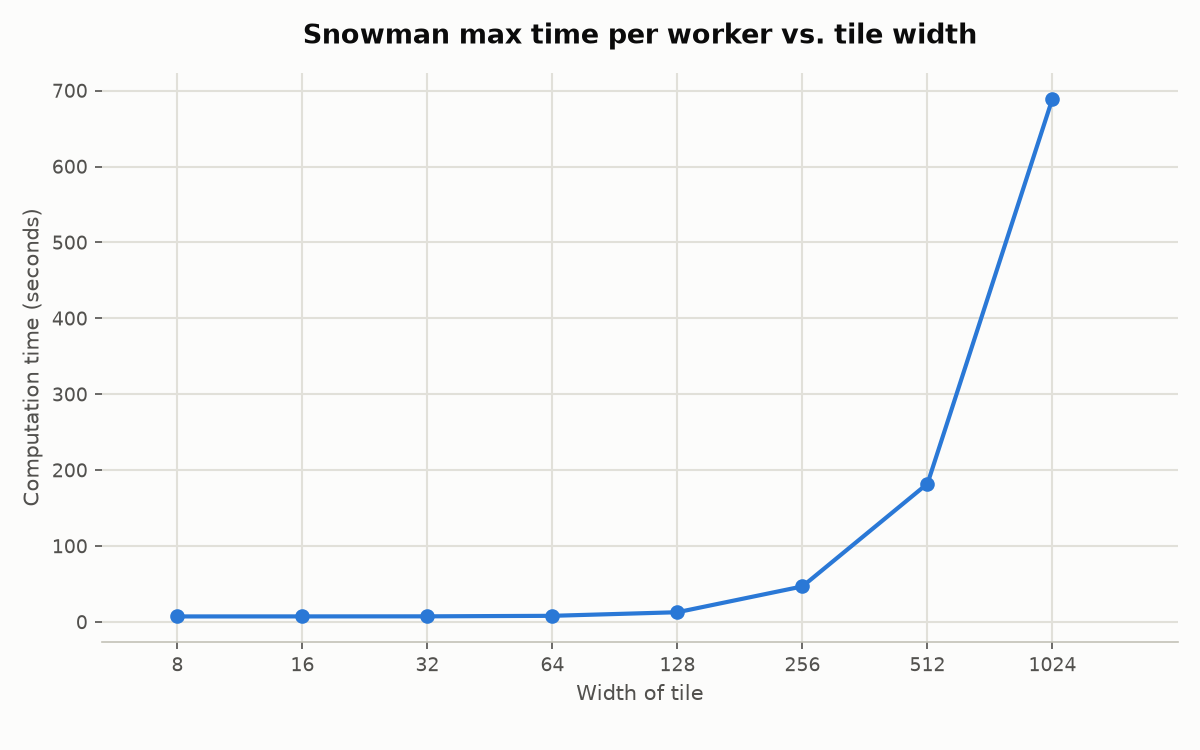
\includegraphics[width=\textwidth]{parts/images/tile_size_ntasks_96.png}
    \caption{Runtime of optimized code on 96 processes for different tile sizes}
\end{figure}

We compared different tile sizes while utilizing a whole node (so 96 workers). The runtime is best for a tile width of 8 pixels (7.31 s) and stays relatively stable up to 64 pixels (8.12 s). The runtime rises dramatically for larger tile sizes. This is to be expected, because there are no longer enough tiles to keep all workers busy. The worst case is a tile width of 1024 pixels (689.52 s). Here, there is just one tile which is the size of the entire image, so the whole image gets processed by one worker. 
\chapter{Conclusion}
We implemented an optimized version of the Snowman application which uses tile decomposition and dynamic scheduling. We could show that our implementation performs better than the unoptimized code when keeping the following considerations in mind:\\
\\
Using dynamic scheduling introduces extra overhead, since there is a master process that does not contribute to actually rendering the image. Therefore, dynamic scheduling does not perform well when using very few processes. Our experiments showed that using eight or more processes with dynamic scheduling led to better performance than the unoptimized implementation. Another important thing to consider is the size of the tiles. It needs to be chosen so that there are enough tiles to keep all workers busy. Our results suggest than when using 96 processes, one should use a tile width of 64 pixels or less. When using less processes, larger tile sizes may be acceptable.\\
\\
Notably, our implementation does not have the "spiky" runtime fluctuations that we saw in the original implementation. This is because of better handling of the remainder when the image size can not be evenly divided by the number of workers. Another problem with the original implementation was that some workers get assigned an entirely white section of the image, while others get sections that are more complex to render. Tile decomposition avoids this issue, which presumably also contributes to some of the speedup we saw.
% EN: Include your content files here
% DE: Füge hier weitere Dateien für deinen Inhalt hinzu


% Bibliography
\clearpage
\bibliography{parts/_bibliography}

% Appendix
\beginClosing
\chapter{\langAppendix}
\begin{longtable}{rrrrrrr}
    \toprule
    & \multicolumn{3}{c}{Unoptimized (baseline)} & \multicolumn{3}{c}{Optimized (tile decomposition)} \\
    \cmidrule(lr){2-4} \cmidrule(lr){5-7}
    Processes & Time (s) & Speedup & Efficiency & Time (s) & Speedup & Efficiency \\
    \midrule
    \endhead
    1 & 688.295 & 1.00 & 100.0\% & -- & -- & -- \\
    2 & 361.156 & 1.91 & 95.3\% & 686.233 & 1.00 & 50.2\% \\
    3 & 239.780 & 2.87 & 95.7\% & 343.209 & 2.01 & 66.8\% \\
    4 & 185.977 & 3.70 & 92.5\% & 228.946 & 3.01 & 75.2\% \\
    5 & 154.095 & 4.47 & 89.3\% & 171.663 & 4.01 & 80.2\% \\
    6 & 129.537 & 5.31 & 88.6\% & 137.597 & 5.00 & 83.4\% \\
    7 & 109.094 & 6.31 & 90.1\% & 114.631 & 6.00 & 85.8\% \\
    8 & 98.921 & 6.96 & 87.0\% & 98.446 & 6.99 & 87.4\% \\
    9 & 86.870 & 7.92 & 88.0\% & 85.988 & 8.00 & 88.9\% \\
    10 & 77.880 & 8.84 & 88.4\% & 76.550 & 8.99 & 89.9\% \\
    11 & 71.178 & 9.67 & 87.9\% & 69.002 & 9.98 & 90.7\% \\
    12 & 65.535 & 10.50 & 87.5\% & 62.649 & 10.99 & 91.6\% \\
    13 & 60.281 & 11.42 & 87.8\% & 57.557 & 11.96 & 92.0\% \\
    14 & 56.054 & 12.28 & 87.7\% & 53.011 & 12.98 & 92.7\% \\
    15 & 52.513 & 13.11 & 87.4\% & 49.394 & 13.93 & 92.9\% \\
    16 & 49.503 & 13.90 & 86.9\% & 46.182 & 14.90 & 93.1\% \\
    17 & 46.314 & 14.86 & 87.4\% & 43.049 & 15.99 & 94.1\% \\
    18 & 43.865 & 15.69 & 87.2\% & 40.815 & 16.86 & 93.7\% \\
    19 & 42.372 & 16.24 & 85.5\% & 38.334 & 17.96 & 94.5\% \\
    20 & 39.373 & 17.48 & 87.4\% & 36.306 & 18.96 & 94.8\% \\
    21 & 38.896 & 17.70 & 84.3\% & 34.746 & 19.81 & 94.3\% \\
    22 & 35.581 & 19.34 & 87.9\% & 32.921 & 20.91 & 95.0\% \\
    23 & 34.110 & 20.18 & 87.7\% & 31.517 & 21.84 & 95.0\% \\
    24 & 34.754 & 19.80 & 82.5\% & 30.184 & 22.80 & 95.0\% \\
    25 & 38.563 & 17.85 & 71.4\% & 28.885 & 23.83 & 95.3\% \\
    26 & 30.168 & 22.82 & 87.8\% & 27.610 & 24.93 & 95.9\% \\
    27 & 37.301 & 18.45 & 68.3\% & 26.771 & 25.71 & 95.2\% \\
    28 & 31.146 & 22.10 & 78.9\% & 25.557 & 26.93 & 96.2\% \\
    29 & 27.095 & 25.40 & 87.6\% & 24.823 & 27.73 & 95.6\% \\
    30 & 26.433 & 26.04 & 86.8\% & 24.084 & 28.58 & 95.3\% \\
    31 & 25.582 & 26.91 & 86.8\% & 23.321 & 29.51 & 95.2\% \\
    32 & 24.770 & 27.79 & 86.8\% & 22.503 & 30.59 & 95.6\% \\
    33 & 23.974 & 28.71 & 87.0\% & 21.555 & 31.93 & 96.8\% \\
    34 & 23.256 & 29.60 & 87.0\% & 21.157 & 32.53 & 95.7\% \\
    35 & 22.658 & 30.38 & 86.8\% & 20.734 & 33.20 & 94.8\% \\
    36 & 26.207 & 26.26 & 73.0\% & 20.044 & 34.34 & 95.4\% \\
    37 & 30.975 & 22.22 & 60.1\% & 19.460 & 35.37 & 95.6\% \\
    38 & 37.439 & 18.38 & 48.4\% & 18.825 & 36.56 & 96.2\% \\
    39 & 21.301 & 32.31 & 82.9\% & 18.186 & 37.85 & 97.0\% \\
    40 & 29.416 & 23.40 & 58.5\% & 18.061 & 38.11 & 95.3\% \\
    41 & 38.315 & 17.96 & 43.8\% & 17.467 & 39.40 & 96.1\% \\
    42 & 23.571 & 29.20 & 69.5\% & 16.857 & 40.83 & 97.2\% \\
    43 & 34.817 & 19.77 & 46.0\% & 16.761 & 41.07 & 95.5\% \\
    44 & 20.637 & 33.35 & 75.8\% & 16.165 & 42.58 & 96.8\% \\
    45 & 33.554 & 20.51 & 45.6\% & 16.091 & 42.78 & 95.1\% \\
    46 & 20.002 & 34.41 & 74.8\% & 15.520 & 44.35 & 96.4\% \\
    47 & 35.038 & 19.64 & 41.8\% & 15.405 & 44.68 & 95.1\% \\
    48 & 22.071 & 31.19 & 65.0\% & 15.064 & 45.69 & 95.2\% \\
    49 & 38.606 & 17.83 & 36.4\% & 15.446 & 44.56 & 90.9\% \\
    50 & 26.333 & 26.14 & 52.3\% & 14.812 & 46.47 & 92.9\% \\
    51 & 15.672 & 43.92 & 86.1\% & 14.748 & 46.67 & 91.5\% \\
    52 & 33.164 & 20.75 & 39.9\% & 14.199 & 48.48 & 93.2\% \\
    53 & 21.331 & 32.27 & 60.9\% & 14.056 & 48.97 & 92.4\% \\
    54 & 42.609 & 16.15 & 29.9\% & 13.994 & 49.18 & 91.1\% \\
    55 & 31.261 & 22.02 & 40.0\% & 13.425 & 51.27 & 93.2\% \\
    56 & 20.193 & 34.09 & 60.9\% & 13.345 & 51.58 & 92.1\% \\
    57 & 43.365 & 15.87 & 27.8\% & 13.228 & 52.03 & 91.3\% \\
    58 & 33.165 & 20.75 & 35.8\% & 12.732 & 54.06 & 93.2\% \\
    59 & 22.762 & 30.24 & 51.3\% & 12.591 & 54.66 & 92.7\% \\
    60 & 13.320 & 51.67 & 86.1\% & 12.581 & 54.71 & 91.2\% \\
    61 & 38.581 & 17.84 & 29.2\% & 12.050 & 57.12 & 93.6\% \\
    62 & 28.502 & 24.15 & 39.0\% & 11.974 & 57.48 & 92.7\% \\
    63 & 18.917 & 36.38 & 57.8\% & 11.909 & 57.80 & 91.7\% \\
    64 & 12.558 & 54.81 & 85.6\% & 11.473 & 60.00 & 93.7\% \\
    65 & 38.718 & 17.78 & 27.3\% & 11.299 & 60.92 & 93.7\% \\
    66 & 29.357 & 23.45 & 35.5\% & 11.240 & 61.24 & 92.8\% \\
    67 & 20.241 & 34.00 & 50.8\% & 11.190 & 61.51 & 91.8\% \\
    68 & 11.703 & 58.82 & 86.5\% & 10.835 & 63.53 & 93.4\% \\
    69 & 43.499 & 15.82 & 22.9\% & 10.742 & 64.08 & 92.9\% \\
    70 & 35.094 & 19.61 & 28.0\% & 10.549 & 65.25 & 93.2\% \\
    71 & 26.042 & 26.43 & 37.2\% & 10.501 & 65.55 & 92.3\% \\
    72 & 17.666 & 38.96 & 54.1\% & 10.399 & 66.19 & 91.9\% \\
    73 & 10.859 & 63.39 & 86.8\% & 10.078 & 68.29 & 93.6\% \\
    74 & 45.630 & 15.08 & 20.4\% & 9.986 & 68.92 & 93.1\% \\
    75 & 37.519 & 18.35 & 24.5\% & 9.826 & 70.05 & 93.4\% \\
    76 & 29.225 & 23.55 & 31.0\% & 9.784 & 70.35 & 92.6\% \\
    77 & 21.534 & 31.96 & 41.5\% & 9.743 & 70.64 & 91.7\% \\
    78 & 13.266 & 51.88 & 66.5\% & 9.412 & 73.13 & 93.8\% \\
    79 & 53.973 & 12.75 & 16.1\% & 9.379 & 73.39 & 92.9\% \\
    80 & 46.564 & 14.78 & 18.5\% & 9.153 & 75.20 & 94.0\% \\
    81 & 38.694 & 17.79 & 22.0\% & 9.097 & 75.66 & 93.4\% \\
    82 & 31.140 & 22.10 & 27.0\% & 9.098 & 75.66 & 92.3\% \\
    83 & 23.921 & 28.77 & 34.7\% & 8.962 & 76.80 & 92.5\% \\
    84 & 16.543 & 41.61 & 49.5\% & 8.755 & 78.62 & 93.6\% \\
    85 & 9.335 & 73.73 & 86.7\% & 8.708 & 79.04 & 93.0\% \\
    86 & 55.007 & 12.51 & 14.5\% & 8.665 & 79.44 & 92.4\% \\
    87 & 47.567 & 14.47 & 16.6\% & 8.433 & 81.62 & 93.8\% \\
    88 & 40.580 & 16.96 & 19.3\% & 8.388 & 82.05 & 93.2\% \\
    89 & 33.453 & 20.58 & 23.1\% & 8.372 & 82.22 & 92.4\% \\
    90 & 26.812 & 25.67 & 28.5\% & 8.238 & 83.55 & 92.8\% \\
    91 & 20.246 & 34.00 & 37.4\% & 8.066 & 85.34 & 93.8\% \\
    92 & 13.584 & 50.67 & 55.1\% & 8.048 & 85.53 & 93.0\% \\
    93 & 8.575 & 80.26 & 86.3\% & 8.029 & 85.72 & 92.2\% \\
    94 & 57.615 & 11.95 & 12.7\% & 7.706 & 89.32 & 95.0\% \\
    95 & 51.500 & 13.36 & 14.1\% & 7.626 & 90.25 & 95.0\% \\
    96 & 44.532 & 15.46 & 16.1\% & 7.652 & 89.95 & 93.7\% \\
    \bottomrule
    \caption{Execution time, speedup and parallel efficiency for all measured process counts: baseline vs.\ optimized}
    \label{tab:strong-scaling-full}
\end{longtable}



\end{document}
